\documentclass[a4paper,12pt]{jsreport}
\usepackage{bm}
\usepackage{ascmac}
\usepackage{amsmath,amssymb}
\usepackage[linesnumbered,ruled,vlined]{algorithm2e}
\usepackage[dvipdfmx]{graphicx}

\usepackage{subfigure}

\begin{document}

\begin{titlepage}

    {\Large 2020年度卒業論文}

    \begin{center}

        \vspace{10truept}

        \vspace*{120truept}

        {\Huge 複数車両同時最適化問題に対する\\$\varepsilon$制約法における\\$\varepsilon$レベル制御法の改良} 
        
        \vspace{100truept}
        
        {\Large 2021年1月27日提出}

        \vspace{50truept}

        {\Large 広島市立大学 情報科学部}
        
        {\Large 知能工学科  計算知能研究室}

        \vspace{10truept}

        {\Large 氏 名   :     松浦 隆斗 (1720189)}

        \vspace{70truept}

        {\Large 指 導: 高濱 徹行  教授}
        
        {\Large \,\ \ \ \ \ \ \ \ \ : 串田 淳一  准教授}
        
        {\Large \,\ \ \ \ \ \ \ \ \ :  原 章   准教授}
        
        \vspace{10truept}

    \end{center}
\end{titlepage}

%目次を出力
\tableofcontents


%自身の論文に合わせて,適時アレンジして用いること.


\chapter{はじめに}
進化的アルゴリズム(Evolutionary Algorithm, EA)は、生物が集団遺伝また進化を繰り返すことで環境に対して最適な状態になる仕組みを模倣して作られた、最適化問題に対して最適解を探索するためのアルゴリズムである。この手法は、ある問題に対して変化と選択に基づく世代交代を繰り返すことで解の集団を進化させ最適解を得る。また、最適化問題は、ある関数が与えられた領域内で最小値または最大値をとるような解を求める問題のことである。

EAは、最適化したい値である目的関数値だけを求める事ができる直接探索法であり、またプログラムの実装も容易である。EAには、遺伝的アルゴリズム(Genetic Algorithm, GA)、進化的戦略(Evolution Strategy, ES)、遺伝的プログラミング(Genetic Programming, GP)などの分類が存在する。また、これらも同じように個体を生物のように捉えることで最適解の探索をしている。

本研究で使用する最適化手法は、上記の戦略ではなく差分進化(Differential Evolution, DE)\cite{DE1}を用いる。DEは、進化的アルゴリズムの一種であり、最適化問題を解く際に用いられる手法である。また、実装が容易であり、優れた探索性能があることから広く使われる手法となっている。
DEは制約なしの最適化手法なので、そのままでは制約付き最適化問題を解くことができない。そのため、これまでにいくつかの制約対処法が提案されている。制約付き最適化問題を制約なし最適化問題にするalpha制約法\cite{α法}などがある。本研究では、制約なし最適化手法を制約付き最適化手法へ変換するアルゴリズム変換法である$\varepsilon$制約法\cite{ε制約法}を用いる。
$\varepsilon$制約法をDEに適用することは容易であり、また特に、DEと$\varepsilon$制約法を組み合わせた$\varepsilon$制約DEは,人工的なベンチマーク問題だけではなく,高次元かつ複数の制約式を持つ実問題においても優れた性能を示すことが報告されている\cite{εDE}。
$\varepsilon$制約法では目的関数と制約逸脱度を分離して最適化することで、2目的の最適化を簡略化している。
$\varepsilon$レベルは制約の緩和度合いを示す値である。この値を初期値から世代の経過とともに徐々に減少させることで、個体群は実行不能領域から実行可能領域へと接近し、最終的に有望な実行可能解を発見できる。$\varepsilon$レベルを制御する際には、そのレベル以下の制約逸脱度を持つ個体が常にある程度存在するように減少させ、0になった後もある程度の最適化を行うことが望ましいとされる\cite{εレベル制御}。
そのため$\varepsilon$制約法では、あらかじめ決定したパラメータによってスケジューリングし、評価回数が上限に達する前に$\varepsilon$レベルを0にするように制御する。
しかしながら、$\varepsilon$制約法には問題の制約式の改善の難易度が反映されていないため、実際に最適化アルゴリズムを実行した際に、あらかじめ決めた$\varepsilon$レベルの減少スケジュールに合わせて探索が進む保証は無い。例えば、制約式の改善が想定よりも難しければ、個体群が実行可能領域に達する前に$\varepsilon$レベルが0になり探索失敗に繋がる。この様な失敗を避けるためには、制約式の改善の難易度を考慮して$\varepsilon$レベルの減少スケジュールを決定する必要がある。しかしながら、各制約式の難易度は探索前には未知であるため、このような方法は困難となる。

そこで本論文では、個体群の探索状況から$\varepsilon$レベルを制御する方法を提案する。提案手法では、従来の減少度合いを決めるパラメータ$cp$の代わりに、現世代の個体群の制約逸脱度から$\varepsilon$レベルの値を決定する。
これにより、$\varepsilon$レベルの制御を個体群の動きに依存させるような制御をし、個体群とε制約法の関連性を作り出すことで、個体群の探索の進度を反映させた$\varepsilon$レベルの制御が可能となる。また、提案手法では本来なら試行錯誤的に決定する$cp$を用いないため、最適化手法としての汎用性を高める効果も期待できる。
対象とする問題は実問題ベースの制約付き最適化問題であるマツダベンチマーク問題とし,探索アルゴリズムにはDEを用いる。

本論文の構成は以下の通りである。第2章では、制約付き最適化問題であるマツダベンチマーク問題について記述する。第3章では、$\varepsilon$DEの先行研究\cite{先行研究}について説明し、第4章では、提案手法である$\varepsilon$レベルを個体群の探索状況にもとづいて$\varepsilon$レベルを制御する方法について説明する。第5章で、実験結果と考察をし、第6章で、本論文のまとめと今後の課題について述べる。


\chapter{マツダベンチマーク問題}
最適化手法を適応させ最適化する問題の一つとして人工的に作成したベンチマーク関数問題があるが、これは実問題を反映した問題であるとは限らない。そこで、環境規制による燃費の向上のための車体重量の軽量化と、顧客ニーズの多様性にともなう多品種少量生産に適応するための共通板厚部品点数の最大化の2目的の制約付き最適化問題であるマツダベンチマーク問題がマツダ株式会社から提案された\cite{マツダベンチマーク問題}。実世界の最適化問題の多くは、多くの制約の下で目的関数の最適値を探索する、制約付き最適化問題であるため、マツダベンチマーク問題は実問題に取り組むうえで重要な問題の一つと言える。

マツダベンチマーク問題は、等式制約を含まない不等式制約条件付き多目的最適化問題であり、目的関数は車の総重量の最小化と共通板厚部品数の最大化となる。設定対象とする車は、車格の異なる3車種、SUV-Car(SUV),Large-Car(CDW),Small-Car(CH5)である。設計変数は、車体の部品の板厚で、制約条件は、正面衝突時の車体の変形量や、事故時の人体に対する影響などを考慮し作られた、安全に乗車できる条件である。本研究では、車の総重量の最小化のみを目的とする単目的ベンチマーク問題とし、以下のように定義する\cite{マツダベンチマーク問題}。
\\
{\large{Design Variables:}}
\begin{eqnarray}
\bm{x}_{SUV}={({x}_1,{x}_2,...,{x}_d)}^T,\\
\bm{x}_{CDW}={({x}_{1+d},{x}_{2+d},...,{x}_{2d})}^T,\\
\bm{x}_{C5H}={({x}_{1+2d},{x}_{2+2d},...,{x}_{3d})}^T,\\
d=74,D=3d\nonumber
\end{eqnarray}
\\
{\large{Minimize:}}
\begin{eqnarray}
{f}_1=Mass(\bm{x}_{SUV})+Mass(\bm{x}_{CDW})+Mass(\bm{x}_{C5H})
\end{eqnarray}

{\large{Subject to:}}
\begin{eqnarray}
{g}_j(\bm{x}_{SUV})\geq0,\\
{g}_{P+j}(\bm{x}_{CDW})\geq0,\\
{g}_{2P+j}(\bm{x}_{C5H})\geq0,\\
j=1,2,...,P,P=18\nonumber\\
SUV:{x}^L_i\leq {x}_i\leq {x}^U_i,\\
SDW:{x}^L_i+d\leq {x}_i+d\leq {x}^U_i+d,\\
C5H:{x}^L_i+2d\leq {x}_i+2d\leq {x}^U_i+2d,\\
i=1,2,...,d,\nonumber\\
{x}^L_i={x}^L_i+d={x}^L_i+2d,{x}^U_i={x}^U_i+d={x}^U_i+2d
\end{eqnarray}

${f}_1$は最小化すべき目的関数であり、車格の異なる3車種、SUV-Car(SUV),Large-Car,Small-Carの総重量である。
設計変数は、各車種独立に74部品の板厚で、ベクトルxの要素数Dは$3d=222$となり、$222$変数の板厚となる。設計要件上の変数の大小関係に関する4個の制約関数と、各車種ごとに応答局面法で算出された14個の制約関数が存在し、3車種それぞれに実験するため、$k=54$種類の制約関数が存在することになる。${x}^L_i$,${x}^U_i(i=1,2,...,D)$は設計変数の下限値、上限値である。さらに、以下ではすべての制約を満足する領域を実行可能解$F$、上下限制限を満足する領域を探索空間$S$とする。



\chapter{$\varepsilon$DEの先行研究}
本章では、$\varepsilon$DEの先行研究\cite{先行研究}について説明する。3.1節では、DEの簡単なアルゴリズムを記述し、3.2節では、$\varepsilon$制約法について説明する。3.3節では、DEに$\varepsilon$制約法を適用させた$\varepsilon$DEについて説明する。また、本研究で用いたベースベクトルの選択戦略を3.4節で説明する。

\section{DEのアルゴリズム}
DEの集団内の各個体は実数値ベクトル$\bm{x}_i=(x_{i1}, \dots, x_{iD})$で表現される。
DEの戦略は,DE$/base/num/cross$として表記される。$base$はベースベクトル$\bm{x}_{r1}$の選択方法,$num$はベースベクトルを変異させるための差分ベクトル
の個数,$cross$ は交叉方法をそれぞれ指定する。

ベースベクトルの選択をrand戦略で$num=1$とし,交叉を2項交叉(binomial crossover) とするDE/rand/1/binのアルゴリズムを以下に示す。

\begin{enumerate}

\item[STEP0:]\mbox{初期化}\\ 
$NP$個の初期個体$\bm{x}_i$を探索空間$\cal{S}$内にランダムに生成し,初期集団$P= \{ \bm{x}_i| i=1,2 \dots ,NP \}$を構築する。

\item[STEP1:]\mbox{終了判定}\\ 
終了条件を満足すれば,アルゴリズムは終了する。

\item[STEP2:]\mbox{突然変異}\\ 
各親個体$\bm{x}_i$に対して,3個体$ \{  \bm{x}_{r1},\bm{x}_{r2},\bm{x}_{r3}  \} $を$\bm{x}_i$および互いに重複しないようにランダムに選択し,式
(\ref{eq:mutation})により変異ベクトル$\bm{v}_i$を生成する。
 \begin{eqnarray}
 \bm{v}_i= \bm{x}_{r1}+ F (\bm{x}_{r2}-\bm{x}_{r3})
\label{eq:mutation}
\end{eqnarray}
ここで,$F$は差分の伸縮を表すスケーリングファクタである。

\item[STEP3:]\mbox{交叉}\\ 
変異ベクトル$\bm{v}_i$を親$\bm{x}_i$と交叉し,子個体$\bm{u}_{i}$を生成する。交叉はbinomial crossoverを用いる。式を以下で示す。
\begin{eqnarray}
\bm{u}_j=
\left\{
\begin{array}{cc}
    \bm{v}_j & \mbox{if$({rand}_j[0,1]\leq CR \vee j={j}_r)$}\\
    \bm{x}_{j,i,g} & \mbox{$otherwise$}\\
\end{array}
\right.
\end{eqnarray}
${rand}_j$は区間$[0,1]$の一様乱数であり、${j}_i$は$[1,D]$区間からランダムに選択した変数番号である。また、$CR$が大きいほど、変異ベクトルの成分が多く$u$に受け継がれる。

なお,子個体$\bm{u}_i$の要素$u_{i,j}$が探索空間 $\cal{S}$外に生成された場合,
以下の方法で修正を行う。
\begin{eqnarray}
u_{i,j} =
\left\{
\begin{array}{ll}
 2x^{L}_j-u_{i,j},  & \mbox{ $u_{i,j} <x^{L}_j $   } \\
  2x^{U}_j-u_{i,j},		   & \mbox{ $u_{i,j} >x^{U}_j $ } \\
\end{array}
\right.
\end{eqnarray}
ここで,$x^{L}_j, x^{U}_j (i = 1, 2, \dots ,D)$ は決定変数$x_j$の下
限値,上限値である。

\item[STEP4:]\mbox{生存選択}\\ 
子ベクトルを評価する。子ベクトル$\bm{u}_{i}$の目的関数値が親$\bm{x}_i$よりも良ければ子ベクトルが生存者となり,親を子ベクトルで置換する。

\item[STEP5:]\mbox{STEP1に戻る。}\\ 

\end{enumerate}



% binomial交叉のアルゴリズム
% algorithm2e というパッケージで書いています.
% https://github.com/Ry0/TeXmemo/tree/master/algorithm2e
% http://tug.ctan.org/macros/latex/contrib/algorithm2e/doc/algorithm2e.pdf


%適時改ページ(\newpage)を入れる
\newpage


\section{$\varepsilon$制約法}
\subsection{制約逸脱度}
$\varepsilon$制約では、個体群が制約をどの程度逸脱しているかを表現するため、制約逸脱度$\phi(\bm x)$を導入する。制約逸脱度$\phi(\bm x)$は、以下を満足する関数である。

\begin{eqnarray}
\left\{
\begin{array}{cc}
    \phi(\bm x)=0(x\in{F})\\
    \phi(\bm x)>0(x\notin{F})\\
\end{array}
\right.
\end{eqnarray}
制約逸脱度度$\phi(\bm x)$には、ペナルティ関数法のペナルティと同様に定義する方法など幾つかの定義の方法があるが、本研究では先行研究で使用していた$\bm{G}(\bm{x})$を解$\bm x$の制約逸脱度ベクトルとして$\phi(\bm x)$を定義する。以下に$\phi(\bm x)$の定義を示す。
\begin{eqnarray}
%\begin{split}
\bm{G(x)}=({G}_1(\bm{x}),{G}_2(\bm{x}),...,{G}_k(\bm{x}))\\   
{G}_i(\bm{x})=
\left\{
\begin{array}{cc}
     |{g}_i(\bm{x})| & \mbox{if${g}_i(\bm{x})<0(i=1,2,...,k)$} \\
    {0} & \mbox{otherwise}\\
\end{array}
\right.\\
{\phi(\bm{x})}=\sum_{i=1}^k {G}_i(\bm{x})
%\end{split}
\end{eqnarray}

\subsection{$\varepsilon$レベル比較}
目的関数値と制約逸脱度の組$(f,\phi)$の集合上において、制約逸脱度が$\varepsilon$以下の場合は目的関数値の大小関係を優先し、それ以外の場合は制約逸脱度の大小関係を優先する比較である$\varepsilon$レベル比較を定義する。点$\bm{x}_1,\bm{x}_2$における関数値を${f}_1,{f}_2$、制約逸脱度を${\phi}_1,{\phi}_2$とすると、通常の大小関係である、$<,\leq$に対応する関数値と制約逸脱度の組$({f}_i,{\phi}_i)$間の大小関係である$\varepsilon$レベル比較${<}_\varepsilon(\varepsilon \geq 0),{\leq}_\varepsilon(\varepsilon \geq 0)$は以下のようになる。
\begin{eqnarray}
({f}_1,{\phi}_1){<}_\varepsilon({f}_2,{\phi}_2)
\Leftrightarrow
\left\{
\begin{array}{cc}
    {f}_1<{f}_2 & \mbox{if ${\phi}_1,{\phi}_2 \leq \varepsilon$}\\
    {f}_1<{f}_2 & \mbox{if ${\phi}_1={\phi}_2$}\\
    {\phi}_1<{\phi}_2 & \mbox{otherwise}\\
\end{array}
\right.
\end{eqnarray}
\begin{eqnarray}
({f}_1,{\phi}_1){\leq}_\varepsilon({f}_2,{\phi}_2)
\Leftrightarrow
\left\{
\begin{array}{cc}
    {f}_1\leq{f}_2 & \mbox{if ${\phi}_1,{\phi}_2 \leq \varepsilon$}\\
    {f}_1\leq{f}_2 & \mbox{if ${\phi}_1={\phi}_2$}\\
    {\phi}_1<{\phi}_2 & \mbox{otherwise}\\
\end{array}
\right.
\end{eqnarray}
なお、${<}_0,{\leq}_0$は制約逸脱度を優先する辞書式比較と一致し、${<}_∞,{\leq}_∞$は目的関数値のみの比較と一致する。


\subsection{$\varepsilon$レベルの制御}
$\varepsilon$レベルの制御の際には、そのレベル以下の個体が常にある程度含まれるようにしながら0まで減少させ、0になった後もある程度の最適化を行うことが望ましい\cite{εレベル制御}。そこで、初期値$\varepsilon(0)$を初期集団の制約逸脱度の良い個体の上位$NP×s(s\in [0,1])$番目の個体の制約逸脱度とし、${T}_0(0<{T}_0<{T}_{max})$世代以降は常に0となるように制御する。世代$t$のベキ乗関数による制御方法を以下に示す。
\begin{eqnarray}
{\varepsilon}(0)=\phi(\bm{x}_\theta)
\end{eqnarray}

\begin{eqnarray}
\varepsilon(t)=
\left\{
\begin{array}{cc}
    {\varepsilon}(0){(1-\frac{t}{T}_0)}^{cp} & \mbox{$0<t<{T}_0$} \\
    {0} & \mbox{$t\geq{T}_0$}\\
\end{array}
\right.
\label{fig:εレベル制御の式}
\end{eqnarray}
ここで、${\bm x}_\theta$は制約逸脱度が上位$NP\times s$番目の個体$(\theta=NP\times s)$とする。${T}_0$は${T}_{max} × r(r\in [0,1])$世代とし、$cp$はベキ乗の係数とする。また、$\varepsilon$レベルの制御の図は4.1節で示す。また、$cp=3$での$\varepsilon$レベルの推移を図\ref{fig:εレベルの動き1}で示す。

\begin{figure}[htbp]
  \centering
  \includegraphics[width=.9\linewidth]{fig3/ipusilon_move1.eps}
  \caption{$\varepsilon$レベルの推移}
  \label{fig:εレベルの動き1}
\end{figure}

\section{$\varepsilon$DEのアルゴリズム}
本節では、$\varepsilon$制約法を適用したDEである$\varepsilon$DEのアルゴリズムを説明する。$\varepsilon$DEの基本的なアルゴリズムはDEと同様であり、$\varepsilon$の制御と$\varepsilon$レベル比較を行う点が異なる。また、$\varepsilon$DEの戦略も通常のDEと同様に、$\varepsilon$DE$/base/num/cross$として表記される。$base$はベースベクトル$\bm{x}_{r1}$の選択方法,$num$はベースベクトルを変異させるための差分ベクトル
の個数,$cross$ は交叉方法をそれぞれ指定する。

ベースベクトルの選択をrand戦略でベースベクトルの選択をrand戦略で$num=1$とし,交叉を2項交叉(binomial crossover) とする$\varepsilon$DE/rand/1/binのアルゴリズムを以下に示す。$\varepsilon$DEのアルゴリズムを以下に示す。
\begin{enumerate}
\item[STEP0:]\mbox{初期化}\\ 
$NP$個の初期個体$\bm{x}_i$を探索空間$\cal{S}$内にランダムに生成し,初期集団$P= \{ \bm{x}_i| i=1,2 \dots ,NP \}$を構築する。

\item[STEP1:]\mbox{終了判定}\\ 
終了条件を満足すれば,アルゴリズムは終了する。

\item[STEP2:]\mbox{突然変異}\\ 
各親個体$\bm{x}_i$に対して,3個体$ \{  \bm{x}_{r1},\bm{x}_{r2},\bm{x}_{r3}  \} $を$\bm{x}_i$および互いに重複しないようにランダムに選択し,式
(\ref{eq:mutation})により変異ベクトル$\bm{v}_i$を生成する。
 \begin{eqnarray}
 \bm{v}_i= \bm{x}_{r1}+ F (\bm{x}_{r2}-\bm{x}_{r3})
\label{eq:mutation}
\end{eqnarray}
ここで,$F$は差分の伸縮を表すスケーリングファクタである。

\item[STEP3:]\mbox{交叉}\\ 
変異ベクトル$\bm{v}_i$を親$\bm{x}_i$と交叉し,子個体$\bm{u}_{i}$を生成する。交叉はbinomial crossoverを用いる。式を以下で示す。
\begin{eqnarray}
\bm{u}_j=
\left\{
\begin{array}{cc}
    \bm{v}_j & \mbox{if$({rand}_j[0,1]\leq CR \vee j={j}_r)$}\\
    \bm{x}_{j,i,g} & \mbox{$otherwise$}\\
\end{array}
\right.
\end{eqnarray}
${rand}_j$は区間$[0,1]$の一様乱数であり、${j}_i$は$[1,D]$区間からランダムに選択した変数番号である。また、$CR$が大きいほど、変異ベクトルの成分が多く$u$に受け継がれる。

なお,子個体$\bm{u}_i$の要素$u_{i,j}$が探索空間 $\cal{S}$外に生成された場合,
以下の方法で修正を行う。
\begin{eqnarray}
u_{i,j} =
\left\{
\begin{array}{ll}
 2x^{L}_j-u_{i,j},  & \mbox{ $u_{i,j} <x^{L}_j $   } \\
  2x^{U}_j-u_{i,j},		   & \mbox{ $u_{i,j} >x^{U}_j $ } \\
\end{array}
\right.
\end{eqnarray}
ここで,$x^{L}_j, x^{U}_j (i = 1, 2, \dots ,D)$ は決定変数$x_j$の下
限値,上限値である。

\item[STEP4:]\mbox{生存選択}\\ 
子個体を評価し、親個体$\bm{x}_i$と$\varepsilon$レベル比較を行う。子個体$\bm{u}_i$が親$\bm{x}_i$よりも良ければ子個体が生存者となり、親を子個体で置換する。

\item[STEP5:]\mbox{$\varepsilon$レベルの制御}\\ 
$\varepsilon$レベル制御関数$\varepsilon(t)$によって、$\varepsilon$レベルを更新する。

\item[STEP6:]\mbox{STEP1に戻る。}\\ 

\end{enumerate}

\subsection{$\varepsilon$DEにおける突然変異戦略}
本論文では、先行研究\cite{先行研究}で使用された、rand戦略とpbest戦略、パレートbest戦略を用いて実験を行う。pbest戦略およびパレートbest戦略を以下で説明する。
\subsubsection{pbest戦略}
pbest戦略は、$\varepsilon$レベル比較により順位付けした個体集団の上位$p$\%の個体群からランダムにベースベクトルを選択する。pbest戦略法によるベースベクトルの選択方法において、上位$NP \times p$個の個体が$\varepsilon$以下である場合、それ以外の場合をそれぞれ図\ref{fig:pbest図}に示す。

\begin{figure*}[htbp]
  \begin{center}
  \subfigure[上位位$NP \times p$個の個体が$\varepsilon$以下である場合]{ 
  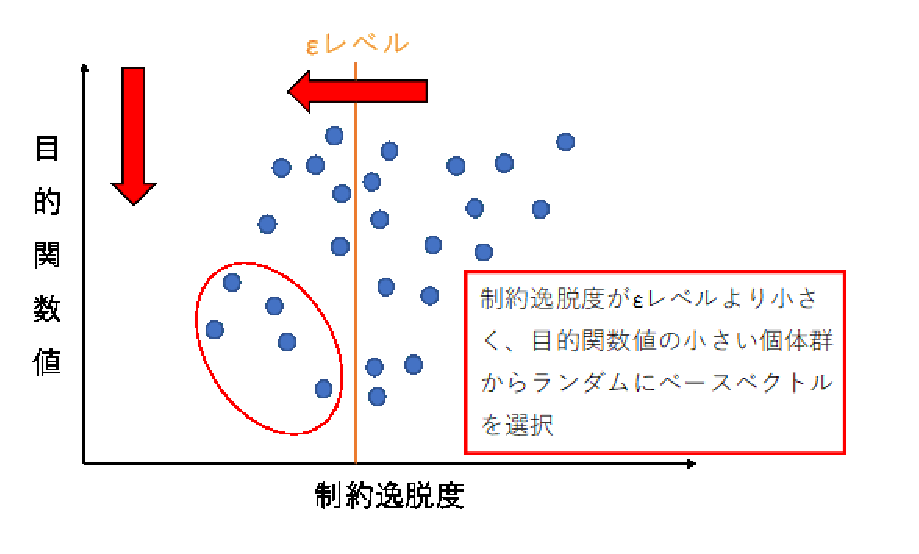
\includegraphics[width=.9\linewidth]{fig3/pbest.eps}
  \label{k11}
  }
  \hfill
  \subfigure[(a)以外の場合]{ 
    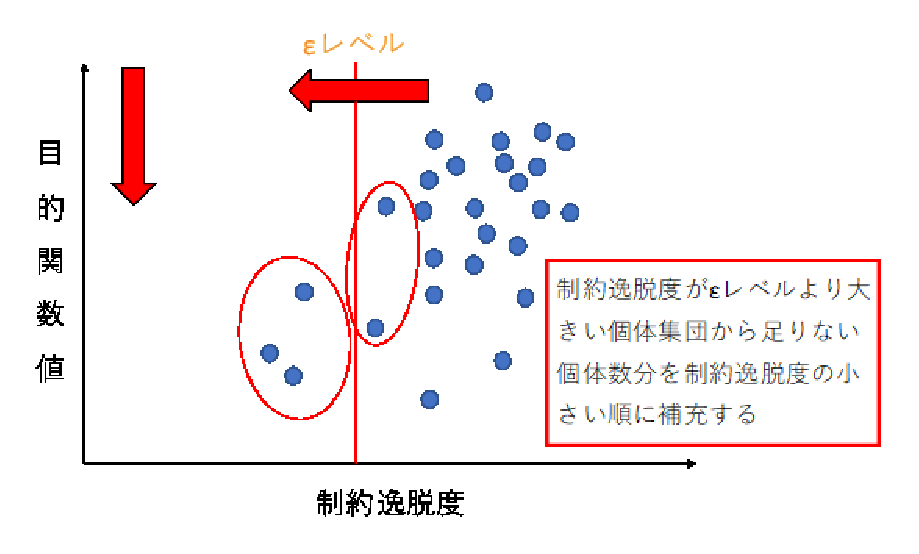
\includegraphics[width=.9\linewidth]{fig3/pbest2.eps}
    \label{k12}
  }
  \end{center}

  \caption{pbest戦略}
  \label{fig:pbest図}
\end{figure*}


\subsubsection{パレートbest戦略}
パレートbest戦略は、各個体において目的関数値、制約逸脱度によって同時に比較し大小関係を決め、個体にランク付けを行う。この比較によって、良い個体集団をランク1とし、ランク1の個体集団からランダムにベースベクトルを選択する。目的関数値と制約逸脱度の同時比較を図\ref{fig:paratebest2}に示す。また、図\ref{fig:paratebest}にパレートbest戦略法による戦略方法を示す。

\begin{figure}[htbp]
  \centering
  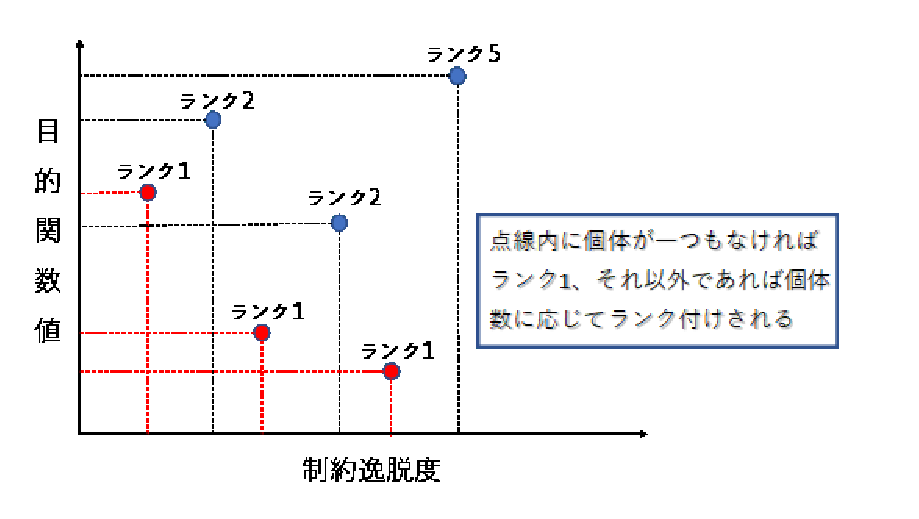
\includegraphics[width=.9\linewidth]{fig3/paratebest2.eps}
  \caption{個体のランク付け}
  \label{fig:paratebest2}
\end{figure}

\begin{figure}[htbp]
  \centering
  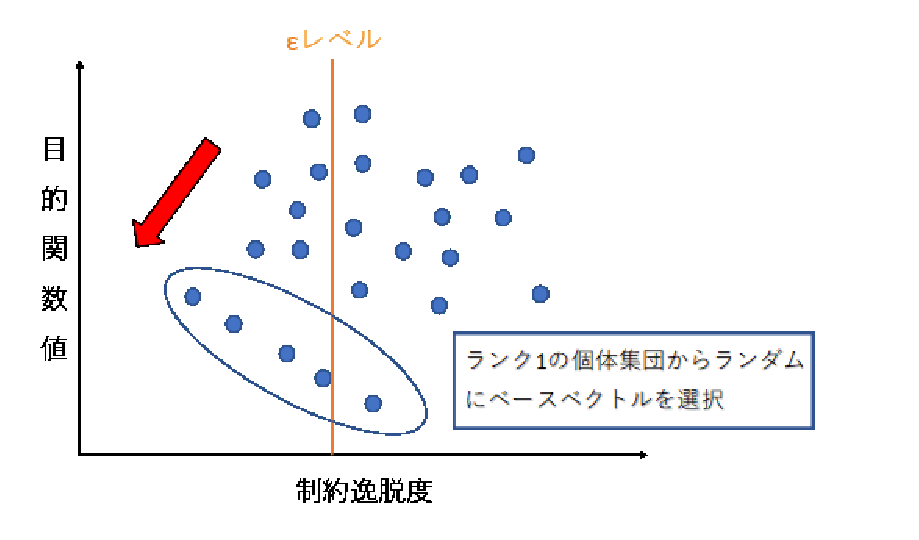
\includegraphics[width=.9\linewidth]{fig3/paratebest.eps}
  \caption{パレートbest戦略}
  \label{fig:paratebest}
\end{figure}


\chapter{提案手法}

$\varepsilon$制約法における$\varepsilon$レベルの制御方法は、あらかじめスケジューリングされていることから、$\varepsilon$制約法には問題の制約式の改善の難易度が反映されていないと考えた。そこで、$\varepsilon$レベルの制御を個体群の動きに依存させるような制御をし、個体集団と$\varepsilon$制約法の関連性を作り出すことで、$\varepsilon$レベルと個体集団の進化度合いの両方を考慮しながら探索を行えるようにする。また、式\ref{fig:εレベル制御の式}より、$\varepsilon$レベルの制御で用いるパラメータ$cp$を用いずに制御することで実験効率を向上を図る。

\section{提案手法の概要}
$\varepsilon$制約のスケジュールをあらかじめ決定せずに個体群の動きに合わしていくように、各世代における個体群の制約逸脱度の良い個体の上位$NP×s$番目の制約逸脱度を$\varepsilon$レベルに代入することで制御する。従来手法では、$s$は$\varepsilon$レベルの初期値を決定するパラメータだったが、提案手法でのパラメータ$s$は、パラメータの使い方を拡張し各世代の$\varepsilon$レベルを決定するときに用いる。
また、個体群の動きに$\varepsilon$レベルを合わせることにより、$\varepsilon$レベルが0に収束する保証がないことから、3.2.3節で記述した${T}_0$を用いることで、あらかじめ決めた世代時に$\varepsilon$レベルが0に達していない場合は制御するようにする。以下のように世代$t$ごとで$\varepsilon$レベルを制御していく。
\begin{eqnarray}
\varepsilon(t)=
\left\{
\begin{array}{cc}
    {\phi({\bm x}_\alpha)} & \mbox{$0\leq t<{T}_0$} \\
    {0} & \mbox{$t\geq{T}_0$}\\
\end{array}
\right.
\label{提案手法}
\end{eqnarray}
ここで、${x}_\alpha$は制約逸脱度が上位$NP×s$番目の個体$(\alpha=NP \times s)$とし、${T}_0$は${T}_{max}\times{r}(r\in[0,1])$世代とする。
個体集団の進化過程において、制約逸脱度が悪化しないことから、$\varepsilon$レベルに以下のような関係が成り立つ。
\begin{eqnarray}
\varepsilon(t) \geq \varepsilon(t+1)
\end{eqnarray}

また、提案手法における各世代の$\varepsilon$レベルのしくみについて図\ref{fig:teian}に示す。

\begin{figure}[htbp]
  \centering
  \includegraphics[width=.9\linewidth]{fig3/teian.eps}
  \caption{提案手法での$\varepsilon$レベルの更新}
  \label{fig:teian}
\end{figure}

\newpage

提案手法では、個体の難易度を考慮し$\varepsilon$レベルを制御しているが、パラメータ設定によって、探索が急速に早まったりする。$T_{0}$世代より早く$\varepsilon$レベルが0に到達した場合、$T_{0}$世代で$\varepsilon$レベルが0に到達していない場合のそれぞれを図\ref{fig:nonipusilon}に示す。図\ref{k22}では、$T_{0}$世代に達した時、$\varepsilon$レベルを強制的に0にする。

\begin{figure*}[htbp]
  \begin{center}
  \subfigure[$T_{0}$世代より早く$\varepsilon$レベルが0に到達した場合]{ 
  \includegraphics[width=.4\linewidth]{fig3/nonipusilon2.eps}
  \label{k21}
  }
  \hfill
  \subfigure[$T_{0}$世代で$\varepsilon$レベルが0に到達していない場合]{ 
    \includegraphics[width=.4\linewidth]{fig3/nonipsilon1.eps}
    \label{k22}
  }
  \end{center}

  \caption{$\varepsilon$レベルの推移}
  \label{fig:nonipusilon}
\end{figure*}





\chapter{実験結果および考察}

\section{実験設定}
本章では、マツダベンチマーク問題に提案手法を適用し、最適化性能と従来手法との比較を分析する。評価回数は、進化計算シンポジウム2017で行われたマツダベンチマーク問題のコンペティションと同様の30000回\cite{評価回数}とする。目的関数の評価回数の上限は30000回であり$NP=50$の場合は、最大世代数${T}_{max}$は600世代となる。rand戦略、pbest戦略、パレートbest戦略、また個体数の変更をし、21試行の実験を行った。各パラメータ設定は、それぞれの戦略において最もよい結果が得られたパラメータとしている。ただし、本論文のマツダベンチマーク問題では$\varepsilon(0)$を初期集団のなかで制約逸脱度の小さい上位$20$\%番目の個体の制約逸脱度とし、${T}_0$は世代数の9割が望ましい\cite{εレベル制御}\cite{先行研究}ことからすべての実験で$r=0.9$とする。

\section{実験結果}
提案手法ではパラメータ$s$の変化による影響が大きく、実験結果が大きく変わってしまう。このことから、まず5.2.1節でパラメータ$s$の特徴について説明する。また、5.2.2節で$\varepsilon$レベルの制御の従来手法との比較をし、提案手法の安定性を示す。5.2.3節、5.2.4節では21試行の実験結果をまとめる。

\subsection{パラメータ$s$の探索性能への影響}
本研究での提案手法では、従来手法の$\varepsilon$レベル制御におけるパラメータ$cp$を用いず、式\ref{提案手法}のようにパラメータ$s$だけを用いて$\varepsilon$レベルの制御をしているので、$s$の変化が実験結果に大きな影響与える。パラメータ$s$を変更し、21試行の実験結果を表\ref{tbl:s}に示す。各パラメータ設定は、$F=0.2,CR=0.4,s \in (1,2,3,4,5,6,7,8,9)$とし、ベースベクトル戦略はrand戦略とする。

\begin{table}[htbp]
\begin{center}
\caption{パラメータ$s$の変化による結果}
\label{tbl:s}
\begin{tabular}{|c|c|c|c|c|c|c|}
\hline
      & Average & Std & Min & Max & Median &  最適解取得回数\\ \hline
s=1 & 2.671024 & 0.014181 & 2.646765 & 2.698084 & 2.669472 & 21 \\ \hline
s=2 & 2.666634 & 0.009525 & 2.647761 & 2.688299 & 2.664439 & 21 \\ \hline
s=3 & 2.670546 & 0.008984 & 2.655048 & 2.688102 & 2.668138 & 21 \\ \hline
s=4 & 2.669272 & 0.013129 & 2.643024 & 2.690942 & 2.672171 & 21 \\ \hline
s=5 & 2.671490 & 0.010203 & 2.649892 & 2.684292 & 2.673080 & 21 \\ \hline
s=6 & 2.665939 & 0.010247 & 2.648905 & 2.695745 & 2.665613 & 21 \\ \hline
s=7 & 2.661406 & 0.012111 & 2.638376 & 2.688706 & 2.662262 & 21 \\ \hline
\bf s=8 &\bf 2.648559 &\bf 0.008984 &\bf 2.632087 &\bf 2.676156 &\bf 2.648801 &\bf 21 \\ \hline
s=9 & 2.599418 & 0.011018 & 2.575046 & 2.615570 & 2.600180 & 0 \\ \hline
\end{tabular}
\end{center}
\end{table}

表\ref{tbl:s}の最適解の平均などからパラメータ$s$は0.8が適していることが分かる。また、$s=0.9$では、実行可能解を得ることができないまま探索が終了していることから$s$は細かな設定が必要であることが分かる。

さらに、パラメータ$s$の変更による影響を見るべく、個体集団の進化推移を以下に示す。パラメータ$s$の設定は、$\varepsilon$制約を満たす個体数と満たしていない個体数を半々とする$s=0.5$、また、表\ref{tbl:s}において良い結果が得られた$s=0.8$、実行可能解を得ることができなかった$s=0.9$とする。
まず$s=0.5$での個体集団の動きを図\ref{fig:graph4}で示す。次に、$s=0.9$での個体集団の動きを図\ref{fig:graph5}、$s=0.8$での個体集団の動きを図\ref{fig:graph6}に示す。実験結果より良い結果を得ることができた$s=0.8$の図を最後に示す。
提案手法では、少なくとも0世代から200世代までに制約を満たす個体を得ることができ、探索速度が速いことから以下の図では、探索初期の0世代,50世代と探索終了である600世代時の個体集団を示している。また、個体数は50個体、rand戦略を使用し、図の赤い線は$\varepsilon$レベル、灰色の線は$\varepsilon$レベル比較による最良個体の軌跡を示している。

\begin{figure*}[htbp]
  \begin{center}
  \subfigure[0世代]{ 
  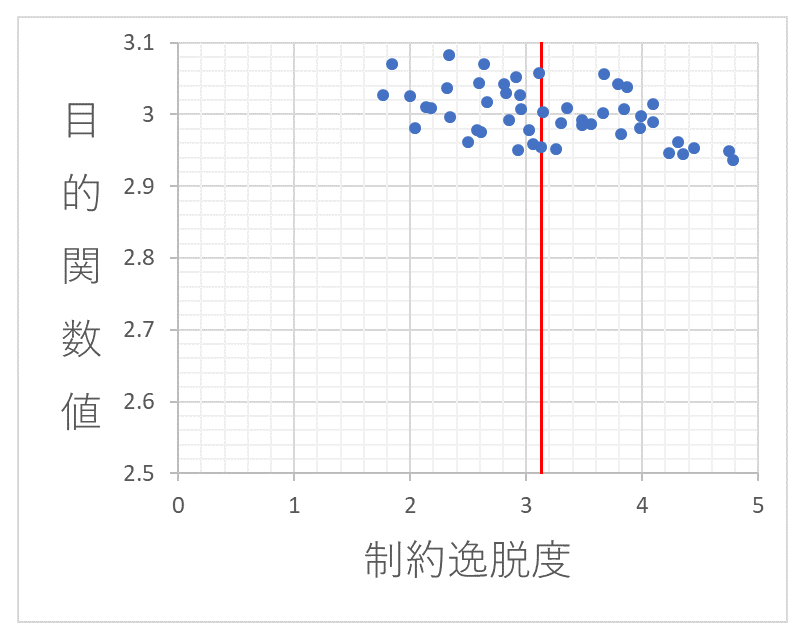
\includegraphics[width=.30\linewidth]{fig3/s=0.5/s=0.5_1.eps}
  \label{k4}
  }
  \hfill
  \subfigure[50世代]{ 
    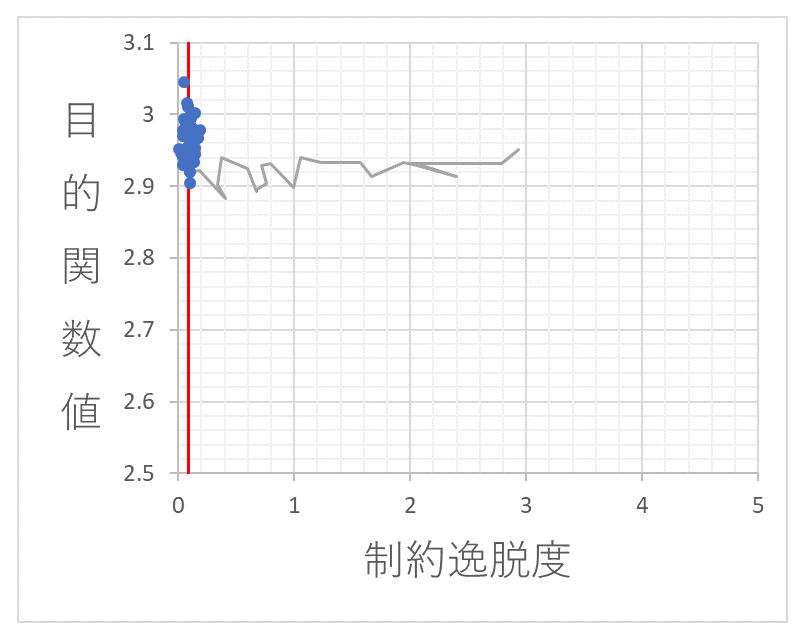
\includegraphics[width=.30\linewidth]{fig3/s=0.5/s=0.5_2.eps}
    \label{k5}
  }
  \hfill
  \subfigure[600世代]{ 
    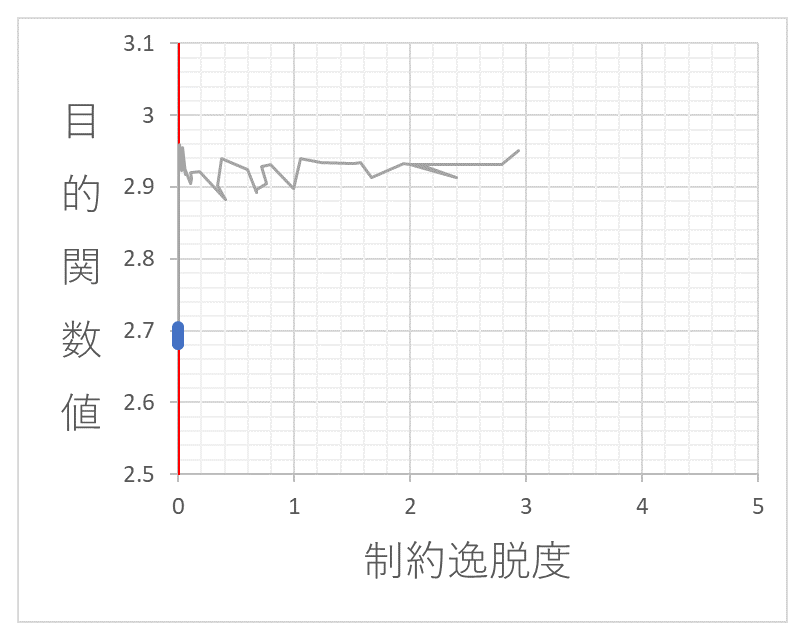
\includegraphics[width=.30\linewidth]{fig3/s=0.5/s=0.5_3.eps}
    \label{k6}
  }
  \end{center}

  \caption{s=0.5}
  \label{fig:graph4}
\end{figure*}

\begin{figure*}[htbp]
  \begin{center}
  \subfigure[0世代]{ 
  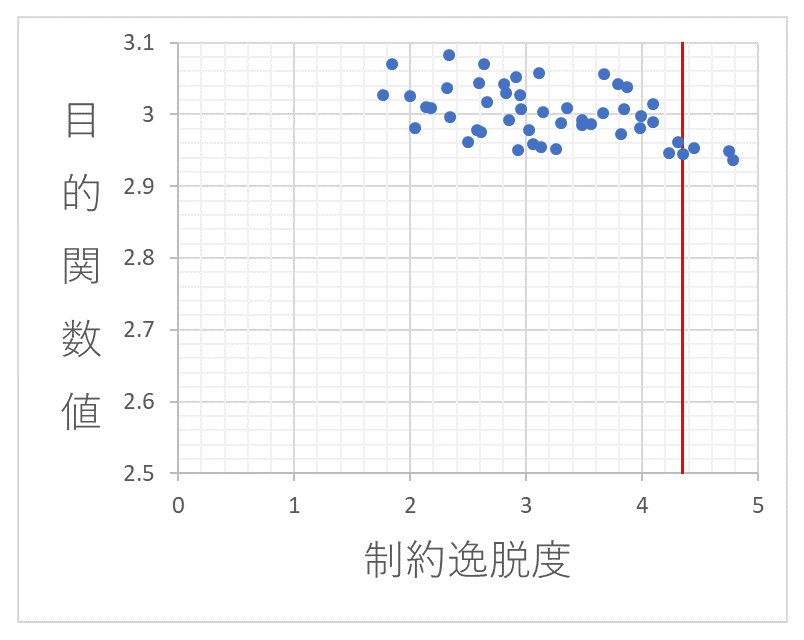
\includegraphics[width=.30\linewidth]{fig3/s=0.9/s=0.9_1.eps}
  \label{k7}
  }
  \hfill
  \subfigure[50世代]{ 
    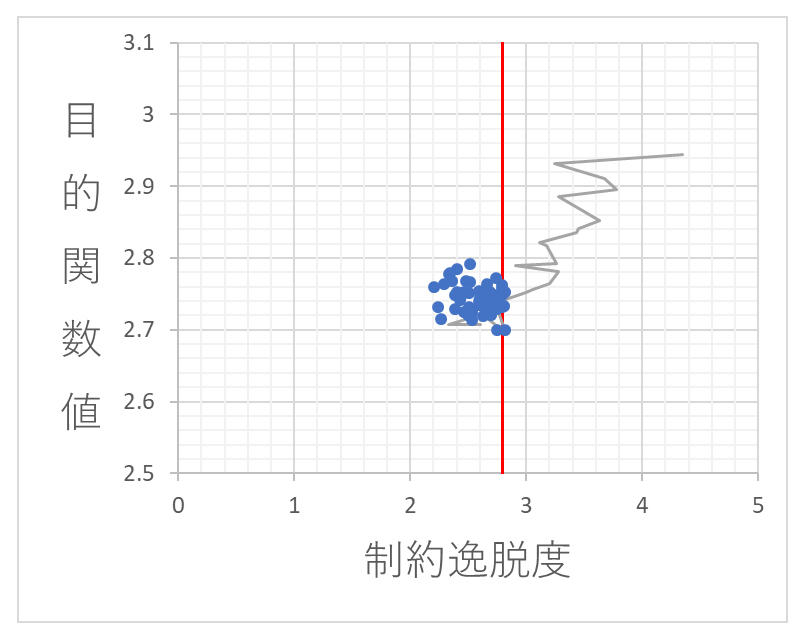
\includegraphics[width=.30\linewidth]{fig3/s=0.9/s=0.9_2.eps}
    \label{k8}
  }
  \hfill
  \subfigure[600世代]{ 
    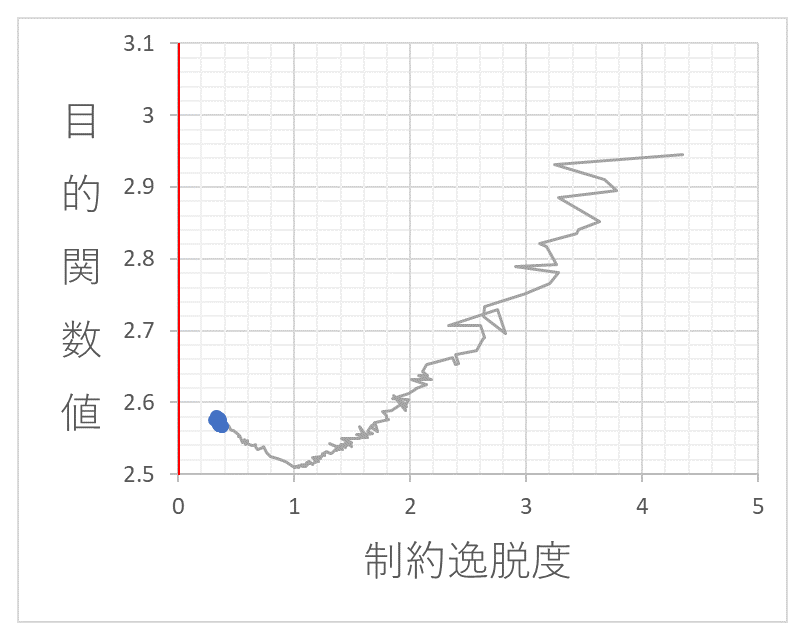
\includegraphics[width=.30\linewidth]{fig3/s=0.9/s=0.9_3.eps}
    \label{k9}
  }
  \end{center}

  \caption{s=0.9}
  \label{fig:graph5}
\end{figure*}

\begin{figure*}[htbp]
  \begin{center}
  \subfigure[0世代]{ 
  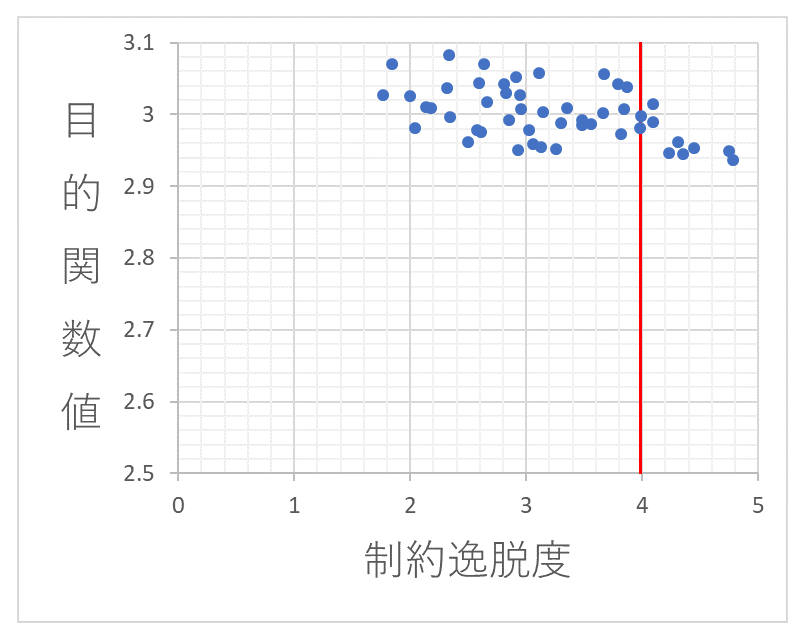
\includegraphics[width=.30\linewidth]{fig3/s=0.8/s=0.8_1.eps}
    \label{k1}
  }
  \hfill
  \subfigure[50世代]{ 
    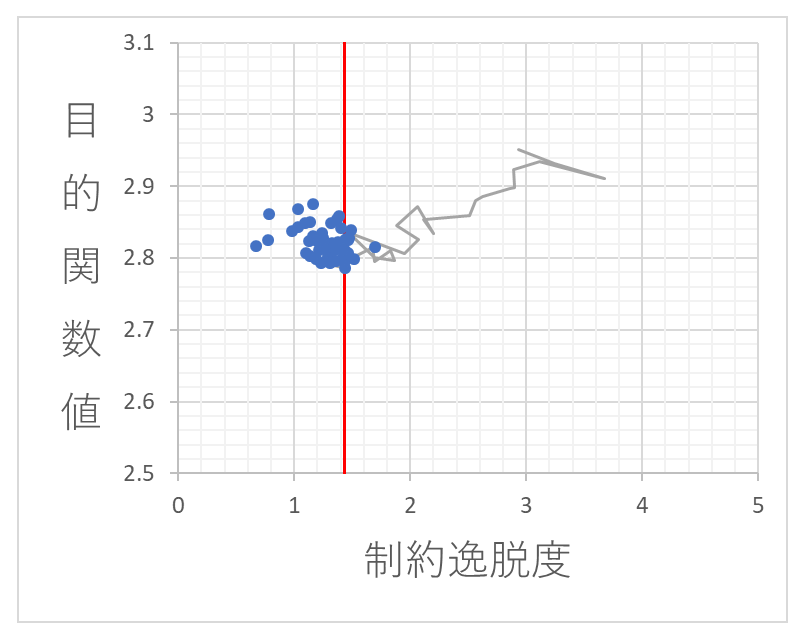
\includegraphics[width=.30\linewidth]{fig3/s=0.8/s=0.8_2.eps}
    \label{k2}
  }
  \hfill
  \subfigure[600世代]{ 
    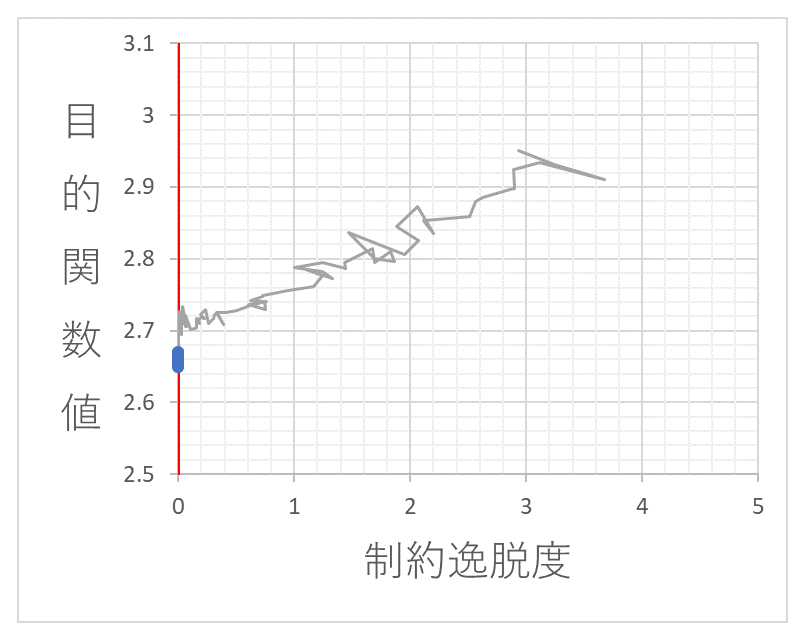
\includegraphics[width=.30\linewidth]{fig3/s=0.8/s=0.8_3.eps}
    \label{k3}
  }
  \end{center}
    
  \caption{s=0.8}
  \label{fig:graph6}
\end{figure*}

図\ref{fig:graph4}では、50世代頃にすでに実行可能領域に接近しており、個体集団が急速に制約を満たすような動きをすることが分かる。また、図\ref{fig:graph5}では、個体集団が急速に目的関数値の良い個体の探索を進め、最終世代までに実行可能領域に達していないことが分かる。図\ref{fig:graph6}では、目的関数値と制約逸脱度のどちらかを改善に偏ることなく、両方をバランスよく探索できているといえる。これらのことから、パラメータ$s$が小さいと制約逸脱度が改善されやすくなり、大きすぎると目的関数値が先に改善され実行可能解を見つけることができない場合が生じることが分かる。パラメータ$s$は、適切な設定をすることで目的関数値と制約逸脱度をバランス良く改善することができることが分かる。

次に、個体集団の進化率からパラメータ$s$の特徴をつかむ。図\ref{fig:evo0.5}、図\ref{fig:evo0.9}、図\ref{fig:evo0.8}はそれぞれ$s=0.5,s=0.9,s=0.8$における各世代での$\varepsilon$制約を満たしている個体と満たしていない個体のそれぞれの進化個体数を示す。


\begin{figure}[htbp]
  \centering
  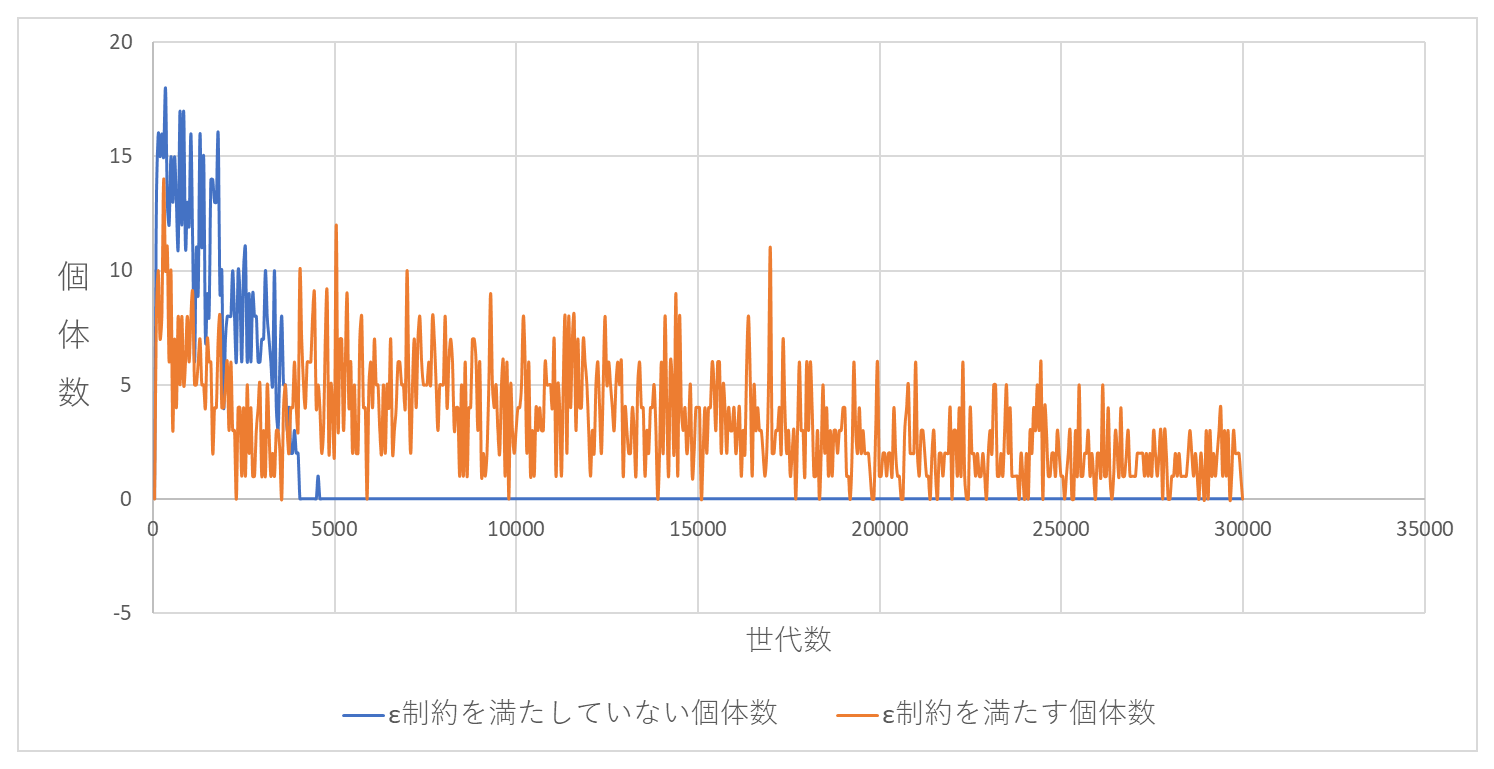
\includegraphics[width=.7\linewidth]{fig3/evo/s=0.5_evo.eps}
  \caption{$s=0.5$における進化個体数}
  \label{fig:evo0.5}
\end{figure}

\begin{figure}[htbp]
  \centering
  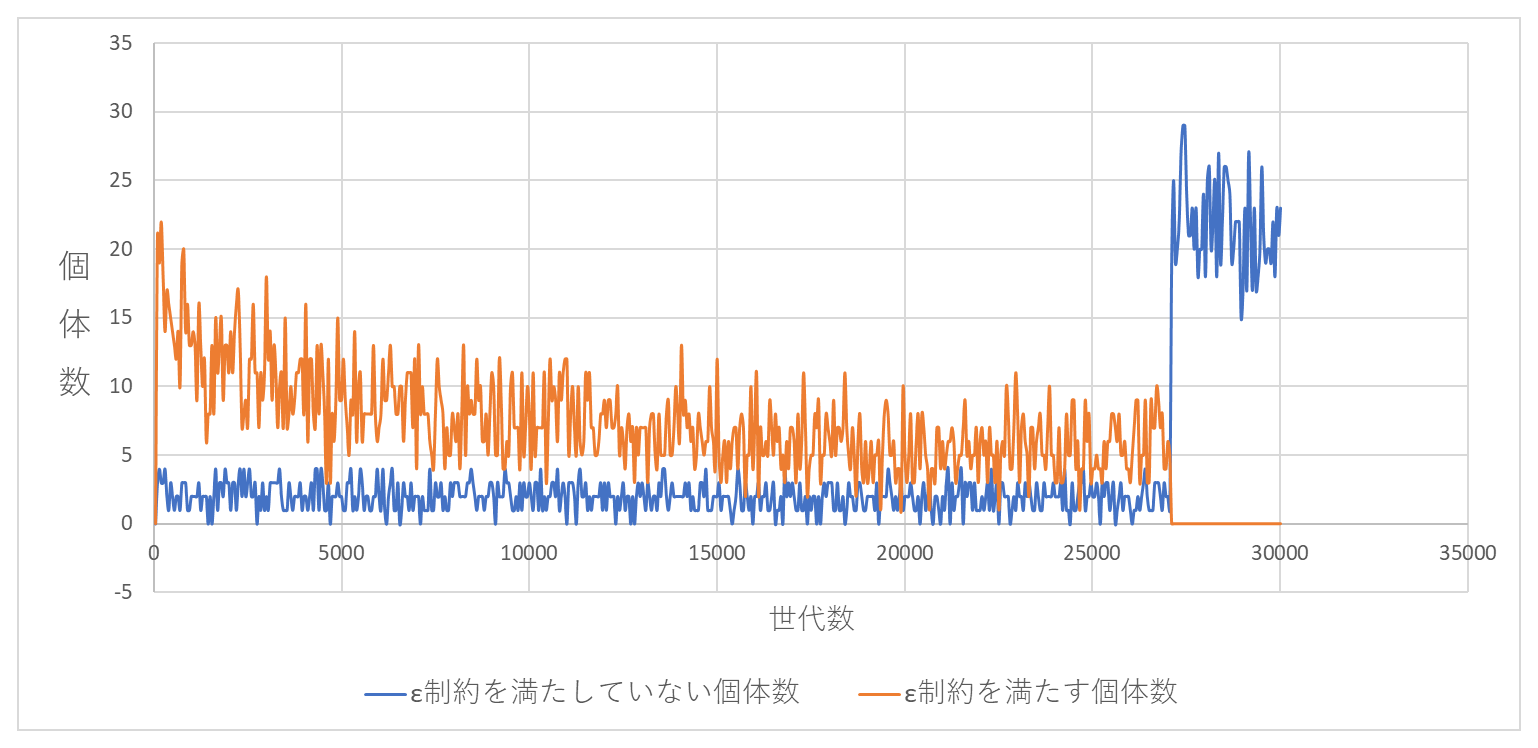
\includegraphics[width=.7\linewidth]{fig3/evo/s=0.9_evo.eps}
  \caption{$s=0.9$における進化個体数}
  \label{fig:evo0.9}
\end{figure}

\begin{figure}[htbp]
  \centering
  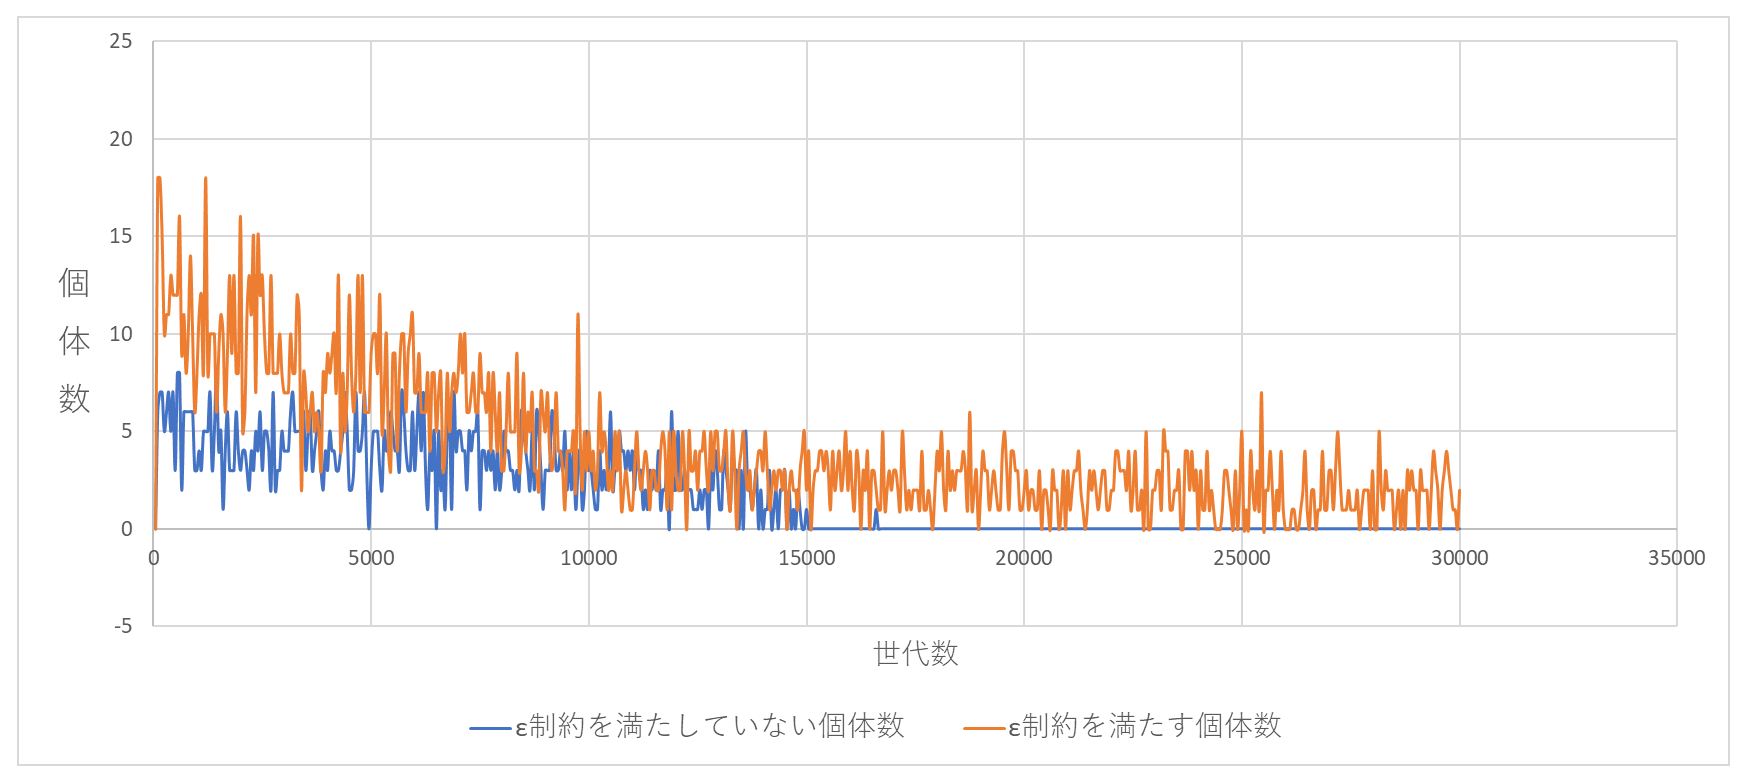
\includegraphics[width=.7\linewidth]{fig3/evo/s=0.8_evo.eps}
  \caption{$s=0.8$における進化個体数}
  \label{fig:evo0.8}
\end{figure}

図\ref{fig:evo0.5}では、$\varepsilon$制約を満たす個体と満たしていない個体の数が同じにも関わらず、$\varepsilon$制約を満たしていない個体の進化率が高いことが分かる。これは、目的関数値よりも制約逸脱度を改善する方が容易であることを示している。また、図\ref{fig:evo0.9}では、$\varepsilon$制約を満たしている個体の進化率に対し、満たしていない個体の進化率が少なすぎることが分かる。そのことから目的関数値の良い個体へと個体集団が進化してしまうと考える。図\ref{fig:evo0.8}は、$\varepsilon$制約を満たす進化率は多いが、満たしていない進化率は比較的に少なくないことが見て取れ、バランスの良い割合で進化しているといえる。また、両方の個体の進化率が同等な時間が多いことも、目的関数値と制約逸脱度の両方をバランス良く改善できた要因だと考える。

上記の結果より、$\varepsilon$制約を満たしている個体の数と満たしていない個体の数の割合によって個体集団の動きに大きく影響が与えられることが分かる。パラメータ$s$は、目的関数値と制約逸脱度の改善のしやすさを考慮して決定する必要があり、具体的には、$s=0.5$に設定し、個体の進化率のバランスを見て、徐々に大きく設定することが良いと考える。
また、$s=0.8$は、実験結果が安定することから、提案手法では$s=0.8$を基準とする。

パラメータ$s$の変化による個体集団の推移をまとめたものを図\ref{fig:s_matome1}、またパラメータ$s$の特徴をまとめたものを図\ref{fig:s_matome2}に示す。

\begin{figure}[htbp]
  \centering
  \includegraphics[width=.7\linewidth]{fig3/s_matome1.eps}
  \caption{パラメータ$s$の変化による個体集団の推移}
  \label{fig:s_matome1}
\end{figure}

\begin{figure}[htbp]
  \centering
  \includegraphics[width=.7\linewidth]{fig3/s_matome2.eps}
  \caption{$s=0.8$における個体の進化推移}
  \label{fig:s_matome2}
\end{figure}

\newpage

\subsection{従来手法と提案手法における$\varepsilon$レベルの変化の比較}
従来手法の$\varepsilon$レベルの制御では、あらかじめ決定されたスケジュールで制御することにより個体集団が実行可能領域に達するようにしているが、提案手法では$\varepsilon$レベルの制御を個体集団の動きに合わすようにしていることから、個体集団が実行可能領域に達する保証がされていない。そこで、従来手法との比較により提案手法での$\varepsilon$レベルの制御が安定性のある制御であることを示す。
ある1試行における提案手法$(s=0.5,s=0.85,s=0.9)$と従来手法で$cp \in       (3,4,5,7,10)$とした場合の$\varepsilon$レベルの変化を図\ref{fig:εレベルの動き1}、図\ref{fig:εレベルの動き}に示す。図\ref{fig:εレベルの動き}の縦軸は制約逸脱度であり対数軸で表示している。また、各パラメータは、$F=0.4,CR=0.5$に設定し、従来手法では$s$は$0.2$で固定し、ベースベクトルの選択戦略はパレートbest戦略とする。このときの最適解を表\ref{tbl:s_cp}に示す。最適解は、表\ref{tbl:s_cp}より、提案手法では$s=0.85$での結果が良く、従来手法の結果と同等の結果が得られている。

\begin{figure}[htbp]
  \centering
  \includegraphics[width=.9\linewidth]{fig3/rebel_move1.eps}
  \caption{$\varepsilon$レベルの動き}
  \label{fig:εレベルの動き1}
\end{figure}

\begin{figure}[htbp]
  \centering
  \includegraphics[width=.9\linewidth]{fig3/rebel_move.eps}
  \caption{$\varepsilon$レベルの動き(縦軸が対数軸)}
  \label{fig:εレベルの動き}
\end{figure}

\begin{table}[htbp]
\begin{center}
\caption{パラメータ$s$とパラメータ$cp$の変化における実験結果}
\label{tbl:s_cp}
\begin{tabular}{|c|c|}
\hline
 s  & 最適解 \\ \hline
 s=0.5 & 2.67053	\\ \hline
 \bf s=0.85 & \bf2.58749 \\ \hline
 s=0.9 & 最適解無し \\ \hline\hline
 cp & 最適解 \\ \hline
 \bf cp=3 & \bf2.58530	\\ \hline
 cp=4 & 2.59623\\ \hline
 cp=5 & 2.58740 \\ \hline
 cp=7 & 2.59498	\\ \hline
 cp=10 & 2.60251 \\ \hline
\end{tabular}
\end{center}
\end{table}

図\ref{fig:εレベルの動き}より、提案手法における$\varepsilon$レベルの下げり方は個体数の進化に合わせるので、従来手法と比較すると不規則な動きなるが、パラメータ$s=0.85$の場合では、$\varepsilon$レベルは0に近づくような動きをすることが分かることから、実行可能解を探索することができる制御といえることができ、特質的な動きが見られないことから安定性もあるといえる。一方、図\ref{fig:εレベルの動き1}からも分かる通り、$s=0.5$の場合では、制約逸脱度を急速に改善しているため$\varepsilon$レベルが急速に減少している。また、$s=0.9$では、$T_{0}$世代までに実行可能領域に達していないため、$\varepsilon$レベルが強制的に0になった結果が分かる。


\subsection{各突然変異における探索性能の比較}
ここでは,提案手法と従来手法において,rand戦略,pbest戦略,パレートbest戦略を適用した際の探索性能を比較する。以下の各戦略においては、従来手法と提案手法ともに21試行すべて実行可能解を見つけることができた結果を示している。
rand戦略を用いた従来手法と提案手法の最適値の平均、標準偏差、最小値、最大値および中央値を表\ref{tbl:rand}に示す。従来手法のパラメータは$F=0.2,CR=0.4,cp=3,s=0.2$、提案手法のパラメータは$F=0.2,CR=0.4,s=0.82$とする。

\begin{table}[htbp]
\begin{center}
\caption{rand戦略}
\label{tbl:rand}
\begin{tabular}{|c|c|c|c|c|c|}
\hline
      & Average & Std & Min & Max & Median  \\ \hline
従来手法 & 2.614087	& 0.007077 & 2.599530 & 2.626882 & 2.614222\\ \hline
提案手法 & 2.631648 & 0.008484 & 2.616347 & 2.645996 & 2.628285\\ \hline
\end{tabular}
\end{center}
\end{table}

pbest戦略を用いた従来手法と提案手法の最適値の平均、標準偏差、最小値、最大値および中央値を表\ref{tbl:pbest}に示す。従来手法のパラメータは$F=0.5,CR=0.9,cp=3,s=0.2$、提案手法のパラメータは$F=0.5,CR=0.9,s=0.8$とする。

\begin{table}[htbp]
\begin{center}
\caption{pbest戦略}
\label{tbl:pbest}
\begin{tabular}{|c|c|c|c|c|c|}
\hline
      & Average & Std & Min & Max & Median  \\ \hline
従来手法 & 2.618152	& 0.007621 & 2.604299 & 2.63508 & 2.617874\\ \hline
提案手法 & 2.628598 & 0.028970 & 2.599050 & 2.743819 & 2.623822\\ \hline
\end{tabular}
\end{center}
\end{table}

パレートbest戦略を用いた従来手法と提案手法の最適値の平均、標準偏差、最小値、最大値および中央値を表\ref{tbl:パレートbest}に示す。従来手法のパラメータは$F=0.4,CR=0.5,cp=3,s=0.2$、提案手法のパラメータは$F=0.4,CR=0.5,s=0.85$とする。

\begin{table}[htbp]
\begin{center}
\caption{パレートbest戦略}
\label{tbl:パレートbest}
\begin{tabular}{|c|c|c|c|c|c|}
\hline
      & Average & Std & Min & Max & Median  \\ \hline
従来手法 & 2.583951	& 0.006241 & 2.572119 & 2.605319 & 2.582695\\ \hline
提案手法 & 2.584854 & 0.003890 & 2.577406 & 2.590795 & 2.585251\\ \hline
\end{tabular}
\end{center}
\end{table}

従来手法との比較の結果、最適値の平均において、すべての戦略で同等の精度を得ることができた。これにより、パラメータ$cp$を減らすことでき、よりシンプルなアルゴリズムとすることができたといえる。また、21試行すべてにおいて実行可能解を得ることができたことから、提案手法によるプログラム変更の影響は少なく、安定性は保たれていると考える。


\subsection{各個体数における探索性能の比較}
従来手法と提案手法において個体数を30個体、40個体、50個体、60個体に変化させた結果から最適値の平均、標準偏差、最小値、最大値および中央値をそれぞれ表\ref{tbl:個体数従来}、表\ref{tbl:個体数提案}に示す。パラメータは、従来手法では、$F=0.4,CR=0.5,cp=3,s=0.2$、提案手法では、$F=0.4,CR=0.5,s=0.85$に設定し実験を行い、どちらも最も良い結果を示している。また、従来手法、提案手法ともに21試行で実行可能解を見つけることができた。
\begin{table}[htbp]
\begin{center}
\caption{従来手法}
\label{tbl:個体数従来}
\begin{tabular}{|c|c|c|c|c|c|}
\hline
      & Average & Std & Min & Max & Median  \\ \hline
30個体 & 2.593698	& 0.016628 & 2.566952 & 2.630099 & 2.587550\\ \hline
\bf40個体 & \bf2.579404 & \bf0.004956 & \bf2.568044 & \bf2.590773 & \bf2.578602\\ \hline
50個体 & 2.583951 & 0.006241 & 2.572119 & 2.605319 & 2.582695\\ \hline
60個体 & 2.588359 & 0.005550 & 2.577464 & 2.600154 & 2.589774\\ \hline
\end{tabular}
\end{center}
\end{table}

\begin{table}[htbp]
\begin{center}
\caption{提案手法}
\label{tbl:個体数提案}
\begin{tabular}{|c|c|c|c|c|c|}
\hline
      & Average & Std & Min & Max & Median  \\ \hline
30個体 & 2.589415	& 0.010051 & 2.576043 & 2.611722 & 2.587608\\ \hline
\bf40個体 & \bf2.580853 & \bf0.005986 & \bf2.570793 & \bf2.593311 & \bf2.581139\\ \hline
50個体 & 2.584854 & 0.00389 & 2.5774060 & 2.590795 & 2.585251\\ \hline
60個体 & 2.588461 & 0.005048 & 2.580141 & 2.599005 & 2.588866\\ \hline
\end{tabular}
\end{center}
\end{table}

個体数の変化による結果から、従来手法、提案手法ともに40個体の結果が最も良い結果が得られた。個体数を減らすことで世代数を増やすことでよい結果が得られたと考えるが、30個体とすると精度は下がる。個体数と世代数のバランスを比較的極端にすることは望ましくないことが分かった。提案手法のパラメータ$s$については、個体数を変更しても$s=0.85$が最も良い結果が得られたことから、少数の個体数変更を行ってもパラメータ$s$は固定できることが分かった。また、個体数を変化させた時のパラメータ$s$の値は、最適化問題ごとにもよるものと考える。






\chapter{おわりに}
本論文では、$\varepsilon$制約法における$\varepsilon$レベルの制御法をあらかじめスケジューリングするのではなく、個体集団の動きに合わすよう改良し、実問題の最適化問題であるマツダベンチマーク問題に適用させ、$\varepsilon$DEの探索性能の向上を図った。

実験結果から従来手法での最適解より良い結果は得ることはできなかったが、パラメータを一つ少なくした上で、従来手法と同等の結果を得ることができた。これは、探索性能の向上は実現できなかったが、アルゴリズムをシンプルにすることができ、今後の実問題に適用される際に実験効率向上になると考える。

また、提案手法ではマツダベンチマーク問題に対して、問題なく最適解を探索することができたが、他の問題に対しても最適解を求める事ができるとは限らない。今後、他の実問題に対しても適用し実験することが必要であると考える。パラメータ$s$も同様であり、戦略ごとでも違う値を設定する必要があることから、問題ごとにも違う値を設定しなければならないと考える。このパラメータ設定も、今後の重要な課題である。


%謝辞には第何章とかの番号をつけなくてもよい.
\chapter*{謝辞}

本研究において,御指導,御教授頂いた高濱徹行教授,串田淳一准教授,原章准教授に
深く感謝致します。


\bibliography{btxsample}
\bibliographystyle{jplain}

%欧文用	和文用	特徴
%plain	jplain	参考文献をアルファベット順で出力する
%unsrt	junsrt	参考文献を引用された順で出力する




\end{document}